% =============================================================
% บทที่ 4 - การวิเคราะห์ ออกแบบ และพัฒนาระบบ
% =============================================================

% -----------------------------------------------------------
\section{การวิเคราะห์ระบบ}
% -----------------------------------------------------------

\subsection{ผังแสดงทิศทางของกิจกรรม (Activity Flow)}

ระบบจำแนกและวิเคราะห์ข่าวสารอัตโนมัติทำงานในลักษณะกระบวนการต่อเนื่อง (Data Pipeline) โดยเริ่มตั้งแต่การดึงข้อมูลจากแหล่งข่าว การประมวลผลและการสกัดข้อมูล การสรุปเนื้อหาและจำแนกหมวดหมู่ ไปจนถึงการบันทึกลงหน่วยจัดเก็บและการกระจายข้อมูลแบบเรียลไทม์ไปยังส่วนติดต่อผู้ใช้ ดังแสดงในผังกิจกรรม (Activity Diagram) ภาพที่ \ref{fig:activity_diagram}

\begin{figure}[H]
\centering
\begin{tikzpicture}[
    node distance=1.1cm and 2.0cm,
    font=\small,
    startstop/.style={draw, circle, fill=black, inner sep=0pt, minimum size=0.4cm},
    endstop/.style={draw, double, circle, fill=black, inner sep=0pt, minimum size=0.4cm},
    activity/.style={draw, rectangle, rounded corners=4pt, minimum width=3.8cm, minimum height=0.8cm, align=center, fill=blue!8, thick},
    decision/.style={draw, diamond, aspect=2, minimum width=2.4cm, minimum height=0.8cm, align=center, fill=yellow!15, thick},
    arrow/.style={thick, ->, >=stealth}
]

% Nodes
\node[startstop] (start) {};
\node[activity, below=0.6cm of start] (scrape) {วนรอบตรวจจับและดึงข่าว\\(Periodic Scraper Trigger)};
\node[activity, below=0.7cm of scrape] (fetch) {ดึงข้อมูลหน้าเว็บ/RSS\\(Playwright / httpx)};
\node[decision, below=0.7cm of fetch] (dup) {ข่าวซ้ำหรือไม่?\\(URL / Hash Check)};
\node[activity, below=0.9cm of dup] (extract) {สกัดเนื้อหาหลักบทความ\\(Trafilatura / BeautifulSoup)};
\node[activity, below=0.7cm of extract] (classify) {ตัดคำ \& จำแนก 9 หมวดหมู่\\(3-Tier Cascade Classifier)};
\node[activity, below=0.7cm of classify] (summarize) {สรุปความ \& วิเคราะห์ Sentiment\\(KKU Gen.AI / Gemini)};
\node[activity, below=0.7cm of summarize] (persist) {จัดเก็บข้อมูลลงระบบ \& แคช\\(Repository \& Multi-tier Cache)};
\node[activity, below=0.7cm of persist] (broadcast) {กระจายสัญญาณข่าวเรียลไทม์\\(Socket.IO \texttt{news:new})};
\node[activity, below=0.7cm of broadcast] (render) {แสดงผลการ์ดข่าว \& In-app Modal\\(Frontend UI)};
\node[endstop, below=0.6cm of render] (end) {};

% Connections
\draw[arrow] (start) -- (scrape);
\draw[arrow] (scrape) -- (fetch);
\draw[arrow] (fetch) -- (dup);
\draw[arrow] (dup) -- node[right] {ไม่ซ้ำ (New)} (extract);
\draw[arrow] (dup.east) -- ++(1.5,0) |- node[near start, right] {ซ้ำ (Cached)} (scrape.east);
\draw[arrow] (extract) -- (classify);
\draw[arrow] (classify) -- (summarize);
\draw[arrow] (summarize) -- (persist);
\draw[arrow] (persist) -- (broadcast);
\draw[arrow] (broadcast) -- (render);
\draw[arrow] (render) -- (end);

\end{tikzpicture}
\caption{แผนภาพแสดงทิศทางกิจกรรมของระบบ (Activity Diagram)}
\label{fig:activity_diagram}
\end{figure}

\subsection{แผนภาพลำดับขั้นตอนการทำงาน (Sequence Diagram)}

การปฏิสัมพันธ์ระหว่างส่วนประกอบต่าง ๆ ของระบบ ตั้งแต่ฝั่งผู้ใช้งาน เว็บเซิร์ฟเวอร์ บริการสเกรปเปอร์ ปัญญาประดิษฐ์ และระบบกระจายข่าว แสดงดังภาพที่ \ref{fig:sequence_diagram}

\begin{figure}[H]
\centering
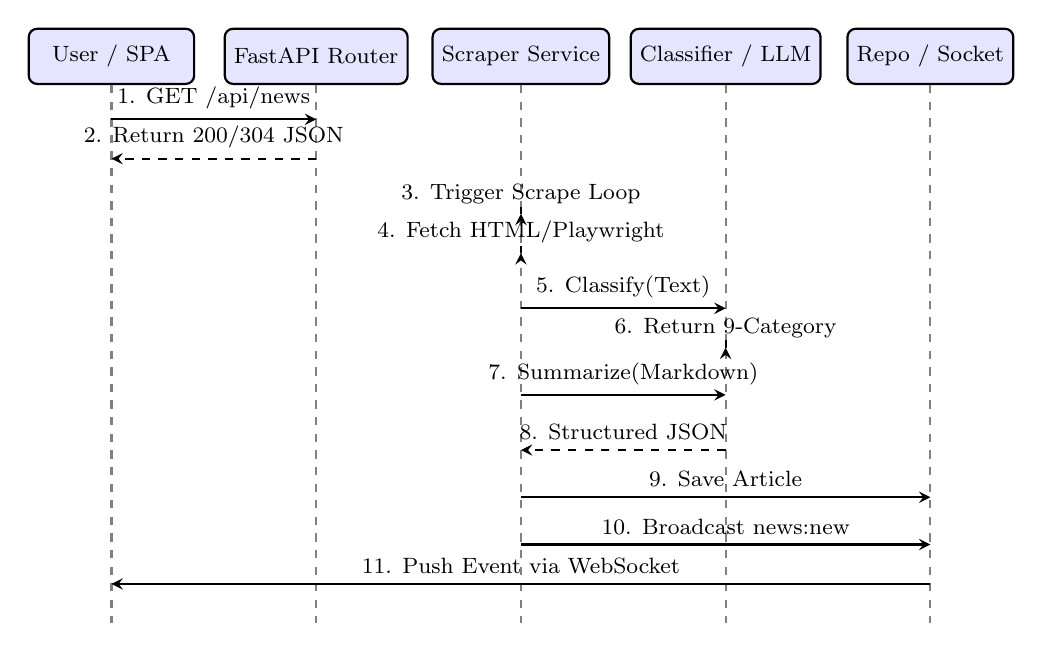
\begin{tikzpicture}[
    font=\footnotesize,
    lifeline/.style={draw, thick, dashed, gray},
    entity/.style={draw, rectangle, rounded corners=3pt, fill=blue!10, thick, minimum width=2.1cm, minimum height=0.7cm, align=center},
    msg/.style={thick, ->, >=stealth},
    retmsg/.style={thick, dashed, ->, >=stealth}
]

% Entities
\node[entity] (u) at (0, 0) {User / SPA};
\node[entity] (r) at (2.6, 0) {FastAPI Router};
\node[entity] (s) at (5.2, 0) {Scraper Service};
\node[entity] (c) at (7.8, 0) {Classifier / LLM};
\node[entity] (db) at (10.4, 0) {Repo / Socket};

% Lifelines
\draw[lifeline] (u) -- (0, -7.2);
\draw[lifeline] (r) -- (2.6, -7.2);
\draw[lifeline] (s) -- (5.2, -7.2);
\draw[lifeline] (c) -- (7.8, -7.2);
\draw[lifeline] (db) -- (10.4, -7.2);

% Messages
\draw[msg] (0, -0.8) -- node[above] {1. GET /api/news} (2.6, -0.8);
\draw[retmsg] (2.6, -1.3) -- node[above] {2. Return 200/304 JSON} (0, -1.3);

\draw[msg] (5.2, -2.0) -- node[above] {3. Trigger Scrape Loop} (5.2, -2.0);
\draw[msg] (5.2, -2.5) -- node[above] {4. Fetch HTML/Playwright} (5.2, -2.5);

\draw[msg] (5.2, -3.2) -- node[above] {5. Classify(Text)} (7.8, -3.2);
\draw[retmsg] (7.8, -3.7) -- node[above] {6. Return 9-Category} (7.8, -3.7);

\draw[msg] (5.2, -4.3) -- node[above] {7. Summarize(Markdown)} (7.8, -4.3);
\draw[retmsg] (7.8, -5.0) -- node[above] {8. Structured JSON} (5.2, -5.0);

\draw[msg] (5.2, -5.6) -- node[above] {9. Save Article} (10.4, -5.6);
\draw[msg] (5.2, -6.2) -- node[above] {10. Broadcast news:new} (10.4, -6.2);
\draw[msg] (10.4, -6.7) -- node[above] {11. Push Event via WebSocket} (0, -6.7);

\end{tikzpicture}
\caption{แผนภาพลำดับขั้นตอนการทำงานของระบบ (Sequence Diagram)}
\label{fig:sequence_diagram}
\end{figure}

\subsection{รายการความต้องการของระบบ}

\subsubsection{ความต้องการเชิงฟังก์ชัน (Functional Requirements)}

ความต้องการเชิงฟังก์ชันของระบบสรุปได้ดังตารางที่ \ref{tab:func_req}

\begin{table}[H]
\centering
\caption{ความต้องการเชิงฟังก์ชันของระบบ (Functional Requirements)}
\label{tab:func_req}
\resizebox{\textwidth}{!}{%
\begin{tabular}{|c|p{4cm}|p{8.5cm}|}
\hline
\textbf{รหัส} & \textbf{ชื่อ Requirement} & \textbf{รายละเอียดความสามารถของระบบ} \\
\hline
FR-01 & Automated Multi-source Scraping & ระบบสามารถดึงข้อมูลข่าวจากแหล่งข่าวออนไลน์หลากหลายแหล่ง ทั้งแบบ RSS Feed, เว็บไซต์ HTML ปกติ และเว็บไซต์ที่เรนเดอร์ด้วย JavaScript ผ่าน Playwright \\ \hline
FR-02 & Dynamic Source Registration & ระบบรองรับการเพิ่ม/ปรับปรุงแหล่งข่าวใหม่ได้อย่างยืดหยุ่นผ่าน Decorator (\texttt{@register\_source}) โดยไม่ต้องแก้ไขโค้ดส่วนประมวลผลหลัก \\ \hline
FR-03 & 9-Category Thai NLP Classification & ระบบสามารถจำแนกหมวดหมู่ข่าวภาษาไทยออกเป็น 9 หมวดหมู่หลักได้อย่างถูกต้องด้วยเทคนิค 3-Tier Cascade Classifier \\ \hline
FR-04 & LLM-Powered Summarization & ระบบสามารถสร้างบทสรุปย่อ ประเด็นสำคัญ และวิเคราะห์อารมณ์ของข่าว (Sentiment) โดยใช้โมเดลภาษาขนาดใหญ่ผ่าน KKU Gen.AI API \\ \hline
FR-05 & Real-time WebSocket Push & ระบบสามารถกระจายข่าวสารใหม่และการอัปเดตสถานะการดึงข่าวไปยังผู้ใช้ทันทีผ่าน Socket.IO โดยผู้ใช้ไม่ต้องรีเฟรชหน้าจอ \\ \hline
FR-06 & Multi-tier Caching & ระบบมีกลไกจัดเก็บแคชในหน่วยความจำ (\texttt{AsyncInMemoryCache}) และแคชแบบมีเงื่อนไข (HTTP 304) เพื่อลดการดึงข้อมูลซ้ำซ้อนและลดภาระเซิร์ฟเวอร์ \\ \hline
FR-07 & Engagement Tracking \& Personalization & ระบบบันทึกพฤติกรรมการใช้งาน (การคลิกอ่าน, การขยายบทสรุป, การบันทึกคั่นหน้า) ผ่านคุกกี้เพื่อนำไปประมวลผลจัดอันดับข่าวที่น่าสนใจ (Trending/Recommended) \\ \hline
FR-08 & In-app Reading Experience & ระบบมีหน้าต่างแสดงผลบทความข่าวและสรุปเนื้อหาในตัวเว็บ (In-app Modal Reader) เพื่อความสะดวกในการอ่าน \\
\hline
\end{tabular}%
}
\end{table}

\subsubsection{ความต้องการที่ไม่ใช่เชิงฟังก์ชัน (Non-Functional Requirements)}

ในด้านความต้องการที่ไม่ใช่เชิงฟังก์ชัน ระบบได้รับการออกแบบให้ตอบสนองข้อกำหนดสำคัญ 4 ประการ ได้แก่ ประการแรก ด้านประสิทธิภาพ (Performance) กำหนดให้เวลาการตอบสนองคำขอเรียกดูรายการข่าวผ่าน REST API (\texttt{GET /api/news}) เฉลี่ยต่ำกว่า 150 มิลลิวินาทีเมื่อมีข้อมูลจัดเก็บในหน่วยความจำแคช และมีอัตราความหน่วงเวลา (Latency) ในการกระจายข่าวสารใหม่ผ่าน WebSocket ต่ำกว่า 500 มิลลิวินาทีนับจากช่วงเวลาที่ข่าวถูกบันทึกลงระบบสำเร็จ ประการที่สอง ด้านความคงทนและการรองรับข้อผิดพลาด (Reliability \& Fault Tolerance) ความล้มเหลวในการดึงข้อมูลจากแหล่งข่าวใดแหล่งข่าวหนึ่งต้องไม่ส่งผลกระทบต่อรอบการทำงานของแหล่งข่าวอื่น (Isolation of Failures) พร้อมทั้งมีกลไกสำรอง (Fallback Mechanism) รองรับการแสดงผลข้อความสรุปพื้นฐานในกรณีที่บริการ LLM ภายนอกขัดข้อง ประการที่สาม ด้านสถาปัตยกรรมและการขยายตัว (Maintainability \& Extensibility) ออกแบบโครงสร้างซอฟต์แวร์ตามหลักการ SOLID และ GRASP โดยแยกชั้นความรับผิดชอบอย่างชัดเจน ตลอดจนการประยุกต์ใช้ Protocol Interface ตามรูปแบบ Port and Adapter Pattern ในการเข้าถึงคลังข้อมูล และประการสุดท้าย ด้านความเป็นส่วนตัวและการรักษาความปลอดภัย (Privacy \& Usability) ระบบยึดหลักการไม่เก็บข้อมูลระบุตัวตนส่วนบุคคล (Non-PII) และมีแถบขอความยินยอมการใช้งานคุกกี้ตามมาตรฐานการคุ้มครองข้อมูลส่วนบุคคล


% -----------------------------------------------------------
\section{การออกแบบระบบ}
% -----------------------------------------------------------

\subsection{สถาปัตยกรรมของระบบและการแบ่งแยกโมดูล (System Architecture)}

ระบบได้รับการออกแบบโครงสร้างสถาปัตยกรรมระดับระบบ (System Architecture Design) สำหรับการติดตั้งบน AWS EC2 \texttt{c7i-flex.large} (2 vCPU, 4 GiB Memory) พร้อมการแยกโมดูลและคอนเทนเนอร์อย่างชัดเจน ดังแสดงในภาพที่ \ref{fig:arch_diagram}

\begin{figure}[H]
\centering
\begin{tikzpicture}[
    font=\small,
    box/.style={draw, rectangle, rounded corners=4pt, fill=blue!5, thick, minimum width=3.5cm, minimum height=1.0cm, align=center},
    container/.style={draw, rectangle, rounded corners=6pt, fill=gray!3, thick, dashed, inner sep=12pt},
    extbox/.style={draw, rectangle, rounded corners=4pt, fill=orange!10, thick, minimum width=3.2cm, minimum height=1.0cm, align=center},
    arrow/.style={thick, <->, >=stealth}
]

% Client Layer
\node[box, fill=green!10] (client) at (0, 4.5) {\textbf{Web Client / SPA}\\Vanilla JS, Tailwind, Socket.IO};

% Server Container
\node[box, fill=purple!10] (nginx) at (0, 2.5) {\textbf{Nginx Reverse Proxy}\\SSL, Static Files, Rate Limit};

\node[box] (router) at (-3.5, 0.5) {\textbf{FastAPI Routers}\\REST API \& Socket.IO};
\node[box] (service) at (0, 0.5) {\textbf{Business Services}\\Scraper, Classifier, LLM};
\node[box] (core) at (3.5, 0.5) {\textbf{Playwright Browser}\\Chromium Headless};

\node[box, fill=cyan!10] (cache) at (-2.0, -1.8) {\textbf{Multi-tier Cache}\\AsyncInMem + HTTP 304};
\node[box, fill=cyan!10] (storage) at (2.0, -1.8) {\textbf{File Repository}\\JSON Storage (Local/S3)};

% AWS EC2 Box
\begin{scope}[on background layer]
    \node[container, fit=(nginx) (router) (service) (core) (cache) (storage), label=above:{\textbf{AWS EC2 Instance (c7i-flex.large: 2 vCPU, 4 GiB Memory)}}] (ec2) {};
\end{scope}

% External APIs
\node[extbox] (llm) at (-4.2, -3.8) {\textbf{KKU Gen.AI Cloud}\\Gemini API Service};
\node[extbox] (sources) at (4.2, -3.8) {\textbf{Online News Sources}\\ThaiPBS, Thairath, RSS};

% Connections
\draw[arrow] (client) -- node[right] {HTTPS / WSS} (nginx);
\draw[arrow] (nginx) -- (router);
\draw[arrow] (router) -- (service);
\draw[arrow] (service) -- (core);
\draw[arrow] (service) -- (cache);
\draw[arrow] (service) -- (storage);
\draw[arrow] (service) -- (llm);
\draw[arrow] (core) -- (sources);

\end{tikzpicture}
\caption{แผนภาพสถาปัตยกรรมระบบและการแบ่งแยกโมดูล (System Architecture Diagram)}
\label{fig:arch_diagram}
\end{figure}

ตารางที่ \ref{tab:arch_layers} แสดงความรับผิดชอบของแต่ละเลเยอร์ในระบบ

\begin{table}[H]
\centering
\caption{การแบ่งชั้นสถาปัตยกรรมของระบบ (Backend Architecture Layers)}
\label{tab:arch_layers}
\resizebox{\textwidth}{!}{%
\begin{tabular}{|l|p{4.2cm}|p{7.2cm}|}
\hline
\textbf{เลเยอร์} & \textbf{โฟลเดอร์/โมดูล} & \textbf{หน้าที่และความรับผิดชอบ} \\
\hline
Presentation & \texttt{frontend/static/} & จัดการหน้าเว็บ Single Page Application (SPA), จัดการ DOM และการรับส่งข้อมูลผ่าน API/WebSocket \\ \hline
Routing & \texttt{backend/routers/} & รับคำขอ HTTP REST API, ตรวจสอบข้อมูลนำเข้า และส่งต่อให้ Service ที่เกี่ยวข้อง \\ \hline
Service (Business Logic) & \texttt{backend/services/} & ควบคุมตรรกะทางธุรกิจ เช่น การรวบรวมข่าว (\texttt{ScraperService}), การสรุปเนื้อหา (\texttt{SummarizerService}), การจำแนกประเภท (\texttt{ClassifierService}), การจัดอันดับความนิยม (\texttt{TrendingService}) \\ \hline
Scraper & \texttt{backend/scrapers/} & สเกรปเปอร์เฉพาะแต่ละแหล่งข่าว ลงทะเบียนด้วย Decorator และฟังก์ชันตัวช่วยแยกวิเคราะห์ HTML \\ \hline
Core / Infrastructure & \texttt{backend/core/} & เครื่องมือส่วนกลาง เช่น \texttt{BrowserService} (Playwright), \texttt{SocketManager}, ระบบแคช (\texttt{AsyncInMemoryCache}) \\ \hline
Persistence & \texttt{backend/repo/} & บันทึกและดึงข้อมูลข่าวและสถิติการใช้งาน (\texttt{FileNewsRepository}, \texttt{FileEngagementRepository}) ตามสัญญา \texttt{NewsRepositoryPort} \\ \hline
Schema & \texttt{backend/schemas/} & กำหนดโครงสร้างข้อมูล (Pydantic Models) สำหรับการแลกเปลี่ยนข้อมูล \\
\hline
\end{tabular}%
}
\end{table}

\subsection{การออกแบบฐานข้อมูลและการจัดเก็บข้อมูล}

โครงสร้างข้อมูลข่าวหลักได้รับการออกแบบให้อยู่ในรูปแบบ JSON Structure ที่กระชับและรองรับการค้นหา ดังแสดงในตารางที่ \ref{tab:news_schema}

\begin{table}[H]
\centering
\caption{โครงสร้างข้อมูลบทความข่าว (\texttt{NewsArticle} Schema)}
\label{tab:news_schema}
\resizebox{\textwidth}{!}{%
\begin{tabular}{|l|l|l|p{6.5cm}|}
\hline
\textbf{ฟิลด์ (Field)} & \textbf{ชนิดข้อมูล} & \textbf{จำเป็น} & \textbf{คำอธิบาย} \\
\hline
\texttt{id} & String & ใช่ & รหัสระบุข่าวแบบไม่ซ้ำ (Hash จาก URL) \\ \hline
\texttt{title} & String & ใช่ & หัวข้อข่าว \\ \hline
\texttt{url} & String & ใช่ & ลิงก์ต้นฉบับบทความข่าว \\ \hline
\texttt{source} & String & ใช่ & ชื่อสำนักข่าวต้นทาง (เช่น ThaiPBS, Thairath, BBC) \\ \hline
\texttt{category} & String & ใช่ & หมวดหมู่ข่าว (politics, economy, tech, etc.) \\ \hline
\texttt{summary} & String & ไม่ใช่ & ข้อความสรุปย่อเนื้อหาข่าวจาก LLM \\ \hline
\texttt{key\_points} & List[String] & ไม่ใช่ & รายการประเด็นสำคัญของข่าว (Bullet points) \\ \hline
\texttt{sentiment} & String & ไม่ใช่ & ค่าอารมณ์ของข่าว (positive, neutral, negative) \\ \hline
\texttt{image\_url} & String & ไม่ใช่ & ลิงก์รูปภาพหน้าปกบทความ \\ \hline
\texttt{published\_at} & String & ใช่ & วันและเวลาที่เผยแพร่ตามมาตรฐาน ISO 8601 \\ \hline
\texttt{created\_at} & String & ใช่ & วันและเวลาที่ระบบนำเข้าข่าว \\ \hline
\texttt{cluster\_id} & String & ไม่ใช่ & รหัสกลุ่มประเด็นข่าวที่รายงานเหตุการณ์เดียวกันข้ามสำนัก \\ \hline
\texttt{consensus\_category} & String & ไม่ใช่ & หมวดหมู่ระดับกลุ่มข่าวที่ผ่านฉันทามติมติเสียงข้างมาก \\ \hline
\texttt{original\_source\_category} & String & ไม่ใช่ & หมวดหมู่ดั้งเดิมที่สำนักข่าวต้นทางระบุไว้เพื่อการตรวจสอบ \\ \hline
\texttt{source\_count} & Integer & ไม่ใช่ & จำนวนสำนักข่าวอิสระที่รายงานข่าวในกลุ่มประเด็นเดียวกัน ($K$) \\
\hline
\end{tabular}%
}
\end{table}

% -----------------------------------------------------------
\section{การพัฒนาระบบและการทำงานของส่วนประกอบหลัก}
% -----------------------------------------------------------

\subsection{กระบวนการดึงข่าวและการเชื่อมต่อ Playwright (Scraping Pipeline)}

ระบบสเกรปข่าวถูกออกแบบให้ทำงานแบบ Asynchronous ทั้งหมด โดยในแต่ละรอบการทำงาน \texttt{ScraperService} จะสร้าง Task สำหรับแต่ละแหล่งข่าวเพื่อดึงข้อมูลพร้อมกัน (Concurrent Scraping) พร้อมทั้งรองรับการดึงหน้าเว็บที่มีการป้องกันด้วย Cloudflare หรือเรนเดอร์เนื้อหาผ่าน JavaScript ผ่าน \texttt{BrowserService} โดยการลงทะเบียนแหล่งข่าวใช้ Decorator \texttt{@register\_source} ดังตัวอย่าง:

\begin{lstlisting}[language=Python, caption={ตัวอย่างการลงทะเบียนแหล่งข่าวด้วย Decorator}]
@register_source("ThaiPBS", "https://www.thaipbs.or.th", "#FF5722")
async def scrape_thaipbs(browser_service: BrowserService) -> list[RawNewsItem]:
    html = await browser_service.fetch_page("https://www.thaipbs.or.th/news")
    return parse_news_cards(html, source="ThaiPBS")
\end{lstlisting}

\subsection{ระบบจำแนกหมวดหมู่และการตัดคำภาษาไทย (Thai NLP Classifier)}

การจำแนกหมวดหมู่ข่าวใช้แนวทางไฮบริด (Hybrid Classification Pipeline) โดยเริ่มต้นจากการสกัดคำสำคัญจากหัวข้อข่าวด้วย PyThaiNLP (\texttt{engine="newmm"}) เพื่อเทียบกับชุดคำศัพท์เฉพาะกลุ่มทั้ง 9 หมวดหมู่หลัก โดยให้ค่าน้ำหนักตามตำแหน่งและความยาวของคำ ในกรณีที่คะแนนจากกฎคำสำคัญไม่ถึงเกณฑ์ความเชื่อมั่นที่กำหนด ระบบจะส่งเวกเตอร์ TF-IDF ของข้อความเข้าสู่โมเดล Support Vector Machine (LinearSVC) ที่ผ่านการเทรนล่วงหน้า และมีโมเดล WangchanBERTa รองรับการประมวลผลข้อความเชิงลึกสำหรับข่าวที่มีบริบทซับซ้อน

\subsection{ระบบเปิดอ่านบทความในตัวเว็บ (In-App Reader) และเอนจินจำลองเบราว์เซอร์ Obscura}

เพื่อยกระดับประสบการณ์การอ่านข่าวให้มีความต่อเนื่องและปลอดภัย ระบบได้พัฒนาหน้าต่างอ่านบทความฉบับเต็มภายในตัวเว็บ (In-App Modal Reader) สำหรับแสดงผลเนื้อหาข่าวที่ผ่านการสกัดและทำความสะอาดแล้ว โดยทำงานร่วมกับ \texttt{BrowserService} และคอนเทนเนอร์ Obscura เมื่อผู้อ่านคลิกเปิดอ่านข่าว ระบบจะตรวจสอบว่ามีเนื้อหา HTML ที่ผ่านการทำความสะอาดแล้วใน \texttt{AsyncInMemoryCache} หรือไม่ หากมีจะส่งกลับทันทีภายในเวลาต่ำกว่า 10 มิลลิวินาที ในกรณีที่เป็นเว็บไซต์ที่เรนเดอร์ด้วย JavaScript ซับซ้อน คอนเทนเนอร์ Obscura จะทำหน้าที่เป็น Headless Browser แยกส่วนเพื่อสกัดเนื้อหาข่าวเบื้องหลังผ่าน Chrome DevTools Protocol (CDP WebSocket \texttt{ws://obscura:9222}) โดยไม่ได้ถูกนำไปรันเป็น In-App Browser ฝั่งผู้ใช้โดยตรง จากนั้นระบบ Backend จะตัดโฆษณา ป้ายแบนเนอร์ แทร็กเกอร์ และองค์ประกอบตกแต่งที่ไม่จำเป็นออกทั้งหมด พร้อมขจัดสคริปต์อันตราย (Anti-XSS) เพื่อความปลอดภัยก่อนส่งไปแสดงผลบนหน้าต่างอ่านข่าว และหากคอนเทนเนอร์ Obscura ไม่ตอบสนองภายในระยะเวลา Timeout ที่กำหนด ระบบจะสลับไปรัน Local Playwright Chromium Engine ภายในตัวแม่ข่ายโดยอัตโนมัติ ทำให้กระบวนการดึงเนื้อหาดำเนินไปได้อย่างต่อเนื่อง

\subsection{ระบบสรุปข่าวอัตโนมัติด้วยโมเดลภาษาขนาดใหญ่ (LLM Summarization Pipeline)}

ระบบส่งเนื้อหาข่าวในรูปแบบ Markdown ให้กับ KKU Gen.AI API โดยออกแบบ Prompt ให้ส่งคืนผลลัพธ์เป็นโครงสร้าง JSON ประกอบด้วย บทสรุปกระชับ 2--3 ประโยค ประเด็นสำคัญ 3--5 ข้อ และการวิเคราะห์อารมณ์ของข่าว (Sentiment: Positive, Neutral, Negative) ในภาษาเดียวกับเนื้อหาต้นฉบับ

\subsection{อัลกอริทึมแนะนำข่าวและจัดอันดับความนิยม (Trending \& Hot News Algorithm)}

การจัดอันดับข่าวติดกระแส (Trending) และข่าวยอดนิยม (Hot News) คำนวณผ่านคลาส \texttt{TrendingService} โดยผสาน 4 ปัจจัยหลัก ได้แก่ คะแนนปฏิสัมพันธ์ของผู้ใช้ (Reader Engagement), ตัวคูณฉันทามติของสำนักข่าว (Multi-source Publisher Consensus Multiplier), การลดทอนตามกาลเวลาแบบครึ่งชีวิต (Half-Life Exponential Time Decay) และคะแนนเร่งพิเศษสำหรับข่าวด่วน (Breaking News Boost)

\subsubsection{สูตรการคำนวณคะแนนความนิยม}

\begin{equation}
\text{TrendingScore} = \left( F_E \times M(K) \times D(\Delta t) \right) + B
\end{equation}

รายละเอียดองค์ประกอบย่อยและหลักการทางทฤษฎีรองรับของแต่ละพจน์ มีดังนี้

พจน์แรกคือ คะแนนปฏิสัมพันธ์ของผู้ใช้แบบลอการิทึม ($F_E$) คำนวณจากผลรวมถ่วงน้ำหนักของพฤติกรรมการอ่าน:
\begin{equation}
E = (1.0 \times N_{\text{clicks}}) + (3.0 \times N_{\text{summaries}}) + (5.0 \times N_{\text{bookmarks}})
\end{equation}
\begin{equation}
F_E = 1.0 + 2.0 \cdot \ln(1.0 + E)
\end{equation}
การคำนวณดังกล่าวได้รับแรงบันดาลใจจากอัลกอริทึมจัดอันดับของ Reddit \cite{salihefendic2010, swartz2005} และ Hacker News \cite{graham2009} ซึ่งใช้ฟังก์ชันลอการิทึมบีบอัดค่าคะแนนตามกฎประโยชน์ส่วนเพิ่มที่ลดน้อยถอยลง (Law of Diminishing Marginal Returns) และป้องกันการปั่นยอดคลิก ทำให้ข่าวที่มียอดคลิกสูงมากจะไม่สามารถครอบครองอันดับได้ตลอดเวลา

พจน์ที่สองคือ ตัวคูณฉันทามติหลายสำนักข่าว ($M(K)$) คำนวณจากจำนวนสำนักข่าวอิสระ $K$ ที่รายงานข่าวในกลุ่มประเด็นเดียวกัน:
\begin{equation}
M(K) = 1.0 + 0.55 \times (K - 1)
\end{equation}
ซึ่งอิงตามทฤษฎี Multi-Source Story Clustering ในระบบ Google News \cite{das2007} โดยถือว่าการที่สำนักข่าวหลายแห่งรายงานตรงกันเป็นตัวบ่งชี้สำคัญว่าเป็นเหตุการณ์สำคัญระดับสาธารณะ

พจน์ที่สามคือ การลดทอนเวลาแบบเอกซ์โพเนนเชียล ($D(\Delta t)$) คำนวณจากระยะเวลา $\Delta t$ ที่ผ่านไปนับจากเวลาเผยแพร่ข่าว:
\begin{equation}
D(\Delta t) = 2^{-\frac{\Delta t}{T_{\text{half}}}}
\end{equation}
โดยอิงตามแบบจำลอง Time-Sensitive Ranking ในงานวิจัยด้าน News Search \cite{dong2010} กำหนดค่าครึ่งชีวิต $T_{\text{half}} = 12.0$ ชั่วโมง ทำให้คะแนนความสดใหม่ลดลงเหลือร้อยละ 50 ทุก 12 ชั่วโมง เพื่อเปิดทางให้ข่าวใหม่ขึ้นมาแสดงแทนที่

และพจน์ที่สี่คือ คะแนนโบนัสข่าวด่วน ($B$) กำหนดขึ้นเพื่อทำหน้าที่เร่งความเร็วข่าวด่วน (Breaking News Velocity Boost) ให้ขึ้นสู่แถบข่าวด่วนทันทีโดยไม่ต้องรอสะสมยอดคลิก:
\begin{equation}
B = \begin{cases} 4.0 & \text{ถ้า } \Delta t \le 3.0 \text{ ชั่วโมง และ } K \ge 2 \\ 0.0 & \text{กรณีอื่น ๆ} \end{cases}
\end{equation}

\subsubsection{เกณฑ์การกำหนดป้ายสถานะ (Badges Thresholds)}
ในการแสดงผลบนส่วนต่อประสานผู้ใช้ ระบบกำหนดเกณฑ์การมอบป้ายสถานะ ได้แก่ ข่าวจะได้รับป้าย [Breaking] เมื่อมีอายุ $\Delta t \le 3.0$ ชั่วโมง และมีสำนักข่าวรายงานตรงกันตั้งแต่ 2 แหล่งขึ้นไป ($K \ge 2$) ได้รับป้าย [Top Story] เมื่อมีสำนักข่าวรายงานตรงกันตั้งแต่ 3 แหล่งขึ้นไป ($K \ge 3$) และได้รับป้าย [Trending] หรือ Hot News เมื่อมีคะแนนรวม $\text{TrendingScore} \ge 4.5$

\subsubsection{ตัวอย่างการคำนวณจริงทีละขั้นตอน (Step-by-Step Numerical Examples)}

เพื่อแสดงการทำงานของอัลกอริทึมอย่างเป็นรูปธรรม จึงยกตัวอย่างการคำนวณ 2 กรณีศึกษา ดังนี้:

\paragraph{กรณีศึกษาที่ 1: ข่าวด่วนที่มีผู้สนใจสูง (Breaking \& Hot Trending News)}
สมมติข่าวอุบัติเหตุใหญ่ที่เพิ่งเผยแพร่ได้ 1.5 ชั่วโมง ($\Delta t = 1.5$) มีรายงานตรงกันจาก 4 สำนักข่าว ($K = 4$) และผู้ใช้งานมีปฏิสัมพันธ์ดังนี้: คลิกอ่าน $N_{\text{clicks}} = 120$ ครั้ง, ขยายอ่านบทสรุป $N_{\text{summaries}} = 45$ ครั้ง, และกดบุ๊กมาร์ก $N_{\text{bookmarks}} = 20$ ครั้ง

\begin{enumerate}[label=\alph*)]
    \item \textit{คำนวณคะแนนปฏิสัมพันธ์:}
    \[ E = (1.0 \times 120) + (3.0 \times 45) + (5.0 \times 20) = 120 + 135 + 100 = 355 \]
    \[ F_E = 1.0 + 2.0 \cdot \ln(1.0 + 355) = 1.0 + 2.0 \cdot \ln(356) = 1.0 + 2.0(5.8749) = 12.75 \]
    
    \item \textit{คำนวณตัวคูณฉันทามติ:}
    \[ M(4) = 1.0 + 0.55(4 - 1) = 1.0 + 1.65 = 2.65 \]
    
    \item \textit{คำนวณอัตราการลดทอนเวลา:}
    \[ D(1.5) = 2^{-\frac{1.5}{12.0}} = 2^{-0.125} \approx 0.9170 \]
    
    \item \textit{คำนวณโบนัสข่าวด่วน:} เนื่องจาก $\Delta t = 1.5 \le 3.0$ และ $K = 4 \ge 2$ ดังนั้น $B = 4.0$
    
    \item \textit{รวมคะแนนสุดท้าย:}
    \[ \text{TrendingScore} = (12.75 \times 2.65 \times 0.9170) + 4.0 = 30.98 + 4.0 = \mathbf{34.98} \]
    \item \textit{ป้ายสถานะที่ได้รับ:} \textbf{[Breaking]}, \textbf{[Top Story]} และ \textbf{[Trending]} (เนื่องจากคะแนน $34.98 \ge 4.5$)
\end{enumerate}

\paragraph{กรณีศึกษาที่ 2: ข่าวเก่าที่มียอดอ่านสูงแต่เสื่อมความนิยมตามเวลา (Older High-Engagement News)}
สมมติข่าวที่เผยแพร่มาแล้ว 36 ชั่วโมง ($\Delta t = 36.0$) รายงานโดยสำนักข่าวเดียว ($K = 1$) แต่สะสมยอดอ่านไว้สูงมาก: $N_{\text{clicks}} = 300, N_{\text{summaries}} = 80, N_{\text{bookmarks}} = 30$

\begin{enumerate}[label=\alph*)]
    \item \textit{คำนวณคะแนนปฏิสัมพันธ์:}
    \[ E = (1.0 \times 300) + (3.0 \times 80) + (5.0 \times 30) = 300 + 240 + 150 = 690 \]
    \[ F_E = 1.0 + 2.0 \cdot \ln(1.0 + 690) = 1.0 + 2.0 \cdot \ln(691) = 1.0 + 2.0(6.5381) = 14.08 \]
    
    \item \textit{คำนวณตัวคูณฉันทามติ:} $M(1) = 1.0 + 0.55(1 - 1) = 1.00$
    
    \item \textit{คำนวณอัตราการลดทอนเวลา:}
    \[ D(36.0) = 2^{-\frac{36.0}{12.0}} = 2^{-3.0} = 0.1250 \]
    
    \item \textit{คำนวณโบนัสข่าวด่วน:} $B = 0.0$ (เนื่องจาก $\Delta t > 3.0$)
    
    \item \textit{รวมคะแนนสุดท้าย:}
    \[ \text{TrendingScore} = (14.08 \times 1.00 \times 0.1250) + 0.0 = \mathbf{1.76} \]
    \item \textit{ผลลัพธ์:} คะแนนลดลงเหลือเพียง 1.76 ทำให้อันดับตกลงและไม่ได้รับป้าย Trending ช่วยเปิดโอกาสให้ข่าวใหม่ที่มีความสดใหม่ขึ้นมาแสดงแทนที่
\end{enumerate}

ตารางที่ \ref{tab:trending_comparison} สรุปเปรียบเทียบผลลัพธ์การคำนวณของทั้งสองกรณีศึกษา

\begin{table}[H]
\centering
\caption{สรุปผลการเปรียบเทียบการคำนวณคะแนน Trending ระหว่างข่าวสดใหม่และข่าวเก่า}
\label{tab:trending_comparison}
\resizebox{\textwidth}{!}{%
\begin{tabular}{|l|c|c|c|c|c|c|l|}
\hline
\textbf{กรณีศึกษา} & $\Delta t$ (ชม.) & $K$ & $F_E$ & $M(K)$ & $D(\Delta t)$ & \textbf{คะแนนสุทธิ} & \textbf{ป้ายสถานะที่ได้รับ} \\
\hline
1. ข่าวด่วนประเด็นร้อน & 1.5 & 4 & 12.75 & 2.65 & 0.9170 & \textbf{34.98} & \textbf{[Breaking]}, \textbf{[Top Story]}, \textbf{[Trending]} \\ \hline
2. ข่าวเก่าสะสมยอดอ่าน & 36.0 & 1 & 14.08 & 1.00 & 0.1250 & \textbf{1.76} & (ไม่มีป้ายสถานะ) \\
\hline
\end{tabular}%
}
\end{table}

\subsection{กระบวนการจัดกลุ่มข่าวจากหลายสำนักข่าวเป็นประเด็นเดียวกัน (Multi-Source Story Clustering Pipeline)}

เพื่อแก้ไขปัญหาการแสดงข่าวซ้ำซ้อนในหมวด Trending และระบุตัวคูณฉันทามติของสำนักข่าว ($K$) ได้อย่างแม่นยำตามข้อเสนอแนะของคณะกรรมการ ระบบได้พัฒนากลไกการรวมข่าวจากหลากหลายสำนักข่าวที่รายงานเหตุการณ์เดียวกันเข้าเป็นกลุ่มประเด็นเดียว (Story Cluster) ผ่าน 3 ขั้นตอนหลัก ดังนี้:

\subsubsection{ขั้นตอนที่ 1: การจำกัดกรอบเวลาการเกิดเหตุการณ์ (Temporal Constraint)}
เนื่องจากข่าวในเหตุการณ์เดียวกันมักเกิดขึ้นและถูกรายงานในเวลาใกล้เคียงกัน บทความข่าว $d_i$ และ $d_j$ จะถูกนำมาพิจารณาจับคู่ก็ต่อเมื่อมีเวลาเผยแพร่ต่างกันไม่เกิน 36 ชั่วโมง:
\begin{equation}
|t_i - t_j| \le 36.0 \text{ ชั่วโมง}
\end{equation}
การจำกัดกรอบเวลาช่วยลดความซับซ้อนในการคำนวณ (Computational Complexity) จากการเปรียบเทียบคู่ข่าวทั้งหมด และตัดข่าวคนละช่วงเวลาที่มีคำศัพท์คล้ายกันออกไปตั้งแต่ขั้นตอนแรก

\subsubsection{ขั้นตอนที่ 2: การวัดความคล้ายคลึงแบบไฮบริดพหุคุณลักษณะ (Multi-Feature Hybrid Similarity)}
การเปรียบเทียบจากหัวข้อข่าวเพียงอย่างเดียวอาจก่อให้เกิดความผิดพลาด เนื่องจากสำนักข่าวแต่ละแห่งอาจรายงานข่าวเดียวกันแต่เขียนคนละมุม (Journalistic Framing) หรือใช้คำคล้ายกันแม้เป็นคนละเหตุการณ์ ระบบจึงใช้ฟังก์ชันความคล้ายคลึงแบบผสมผสาน 4 คุณลักษณะ:
\begin{equation}
\text{Sim}(d_i, d_j) = w_1 \cdot \text{Sim}_{\text{Title}} + w_2 \cdot \text{Sim}_{\text{Summary}} + w_3 \cdot \text{Sim}_{\text{Entities}} + w_4 \cdot \text{Sim}_{\text{Keywords}}
\end{equation}
โดยกำหนดน้ำหนัก $w_1 = 0.35$ (หัวข้อข่าว), $w_2 = 0.30$ (บทสรุปย่อจาก LLM), $w_3 = 0.20$ (เอนทิตีชื่อเฉพาะ) และ $w_4 = 0.15$ (คำสำคัญ) ในส่วนของ $\text{Sim}_{\text{Title}}$ และ $\text{Sim}_{\text{Summary}}$ จะคำนวณความคล้ายคลึงเชิงความหมาย (Semantic Cosine Similarity) ของเวกเตอร์ TF-IDF หรือ Sentence Embeddings เพื่อจับคู่เนื้อหาแม้จะใช้สำนวนภาษาที่แตกต่างกัน สำหรับ $\text{Sim}_{\text{Entities}}$ อาศัยการสกัดชื่อบุคคล สถานที่ และองค์กรที่เกี่ยวข้องผ่านเอนจิน NER ของ PyThaiNLP และคำนวณสัดส่วนการทับซ้อนตามสมการ:
\begin{equation}
\text{Sim}_{\text{Entities}} = \frac{|E_i \cap E_j|}{|E_i \cup E_j|}
\end{equation}
หากมีชื่อบุคคลสำคัญหรือสถานที่เกิดเหตุเดียวกัน ปัจจัยนี้จะช่วยยืนยันความถูกต้องว่าเป็นเหตุการณ์เดียวกันอย่างแม่นยำ และ $\text{Sim}_{\text{Keywords}}$ เปรียบเทียบสัดส่วนของชุดคำสำคัญเฉพาะประเด็น ทั้งนี้ หากค่าความคล้ายคลึงรวม $\text{Sim}(d_i, d_j) \ge \theta_{\text{cluster}}$ (โดยกำหนดค่าขีดเริ่มเปลี่ยน $\theta_{\text{cluster}} = 0.65$) ระบบจะรวมบทความทั้งสองเข้าเป็นกลุ่มข่าวเดียวกัน

\subsubsection{ขั้นตอนที่ 3: การคัดเลือกข่าวตัวแทนกลุ่มและการแสดงผล (Representative Selection \& UI Display)}
เมื่อจัดกลุ่มบทความสำเร็จ ระบบจะคัดเลือกบทความข่าวที่มีคะแนน $\text{TrendingScore}$ สูงสุดในกลุ่มขึ้นมาเป็นข่าวตัวแทนหลักสำหรับแสดงบนการ์ดข่าวหน้าแรก พร้อมทั้งแสดงป้ายระบุจำนวนสำนักข่าวที่รายงานร่วมกันอย่างเด่นชัด เช่น \texttt{[รายงานโดย 4 สำนักข่าว]} และระบุรายชื่อสำนักข่าวต้นทางทั้งหมด เพื่อให้ผู้ใช้สามารถคลิกเปิดอ่านมุมมองข่าวฉบับเต็มของแต่ละสำนักได้อย่างสะดวก

\subsection{การแก้ไขความขัดแย้งของหมวดหมู่ข่าวและการหาฉันทามติระดับกลุ่ม (Cluster-Level Category Consensus)}

ปัญหาสำคัญประการหนึ่งในการรวมข่าวสารจากหลายสำนัก คือความไม่สอดคล้องของหมวดหมู่ข่าว (Category Discrepancy) เนื่องจากแต่ละสำนักข่าวอาจกำหนดโครงสร้าง URL หรือ Tag หมวดหมู่ต่างกันสำหรับข่าวเหตุการณ์เดียวกัน เพื่อแก้ไขปัญหานี้ ระบบได้ออกแบบกลไกการหาฉันทามติหมวดหมู่ระดับกลุ่ม โดยเริ่มต้นจากการใช้มติเสียงข้างมาก (Majority Voting Consensus) เพื่อนับคะแนนหมวดหมู่ที่ทำนายได้จากทุกบทความภายในกลุ่มข่าวเดียวกัน:
\begin{equation}
C^* = \arg\max_{c \in \mathcal{C}} \sum_{d_k \in \text{Cluster}} \mathbb{I}(\text{category}(d_k) = c)
\end{equation}
โดยหมวดหมู่ $c$ ที่ได้รับเสียงสนับสนุนจากสำนักข่าวมากที่สุด จะถูกกำหนดให้เป็นหมวดหมู่ทางการของกลุ่มข่าว (\texttt{consensus\_category}) เพื่อใช้ในการจัดหมวดหมู่และกรองข่าวบนหน้าเว็บ และในกรณีที่คะแนนเสียงข้างมากมีค่าเท่ากัน ระบบจะนำข้อความสรุปย่อรวมของทั้งกลุ่มส่งเข้าสู่โมเดล 3-Tier Cascade Classifier (TF-IDF + LinearSVC / WangchanBERTa) เพื่อวิเคราะห์บริบทของเนื้อหาทั้งหมดและตัดสินหมวดหมู่ที่แท้จริง ทั้งนี้ ระบบยังคงเก็บรักษาฟิลด์ \texttt{original\_source\_category} ดั้งเดิมของแต่ละสำนักข่าวไว้ในฐานข้อมูล เพื่อความโปร่งใสและสามารถตรวจสอบย้อนหลังได้ (Audit Trail)

\subsection{การติดต่อสื่อสารแบบเรียลไทม์ผ่าน WebSocket}

เมื่อมีข่าวใหม่ที่ผ่านการสรุปและจำแนกเรียบร้อยแล้ว \texttt{SocketManager} จะทำการกระจาย Event (\texttt{news:new}) ไปยังเบราว์เซอร์ของผู้ใช้ทุกคนที่กำลังเปิดหน้าเว็บอยู่ เพื่อให้ผู้ใช้ได้รับข่าวสารล่าสุดทันทีโดยไม่ต้องทำการรีเฟรชหน้าต่างเบราว์เซอร์

% -----------------------------------------------------------
\section{การออกแบบและมาตรการความมั่นคงปลอดภัยของระบบ (System Security Design)}
% -----------------------------------------------------------

ความมั่นคงปลอดภัยของระบบ (System Security) และการคุ้มครองความเป็นส่วนตัวของผู้ใช้งาน (Data Privacy) เป็นปัจจัยสำคัญในการพัฒนาเว็บแอปพลิเคชันยุคใหม่ โดยระบบได้ออกแบบมาตรการรักษาความปลอดภัยครอบคลุม 4 มิติหลัก ดังนี้

\subsection{ความมั่นคงปลอดภัยระดับเครือข่ายและเว็บเซิร์ฟเวอร์ (Network \& Gateway Security)}

ในระดับเครือข่าย ระบบได้ติดตั้ง Nginx Reverse Proxy ทำหน้าที่เป็น Gateway จัดการเข้ารหัสช่องทางการสื่อสาร (TLS/SSL Encryption) ทั้งในรูปแบบ HTTPS และ Secure WebSocket (WSS) เพื่อป้องกันการดักฟังข้อมูลระหว่างทาง (Man-in-the-Middle Attack) พร้อมทั้งกำหนดนโยบายจำกัดอัตราการเรียกใช้งาน (API Rate Limiting) เพื่อจำกัดจำนวนคำขอต่อหมายเลข IP ช่วยป้องกันการโจมตีแบบปฏิเสธการให้บริการ (DoS) นอกจากนี้ยังได้กำหนดนโยบายการเข้าถึงข้ามโดเมน (CORS Whitelist) เฉพาะโดเมนของระบบที่ได้รับอนุญาต และติดตั้งส่วนหัวความปลอดภัยมาตรฐาน (HTTP Security Headers) ได้แก่ \texttt{X-Content-Type-Options: nosniff}, \texttt{X-Frame-Options: SAMEORIGIN} และ \texttt{Content-Security-Policy (CSP)} เพื่อป้องกันการโจมตีแบบ Clickjacking และ MIME Confusion

\subsection{การป้องกันการฉีดโค้ดอันตรายและการตรวจสอบข้อมูล (Data Sanitization \& Injection Defense)}

ในด้านการป้องกันการโจมตีเชิงความปลอดภัยและการจัดการข้อมูลอันตราย ระบบมีมาตรการป้องกันที่ครอบคลุมหลายระดับ โดยสำหรับการป้องกัน Cross-Site Scripting (XSS) ข้อมูลเนื้อหาข่าวที่สกัดได้จากเว็บต้นทางอาจมีแท็ก HTML หรือสคริปต์อันตรายแฝงมา ระบบจึงใช้กระบวนการแปลงและกรองข้อมูล (Sanitization) เพื่อกำจัดแท็ก \texttt{<script>}, \texttt{<iframe>}, รวมถึงแอตทริบิวต์ \texttt{onload}, \texttt{onerror} ออกทั้งหมด และแปลงเนื้อหาให้อยู่ในรูป Plain Markdown ก่อนส่งไปแสดงผลบนหน้าจอ In-app Modal นอกจากนี้ เพื่อป้องกันข้อผิดพลาดจาก Malformed Input และ Parameter Tampering ระบบได้บังคับใช้การตรวจสอบโครงสร้างข้อมูลเข้มงวดด้วย Pydantic (Strict Schema Validation) ในทุกจุดรับเข้าและส่งออกของ REST API

สำหรับการป้องกัน Server-Side Request Forgery (SSRF) ส่วนงาน Scraper และ Playwright Service จะรับคำขอและดึงข้อมูลเฉพาะจากรายการสำนักข่าวที่ลงทะเบียนไว้ล่วงหน้า (Source Whitelist) เท่านั้น โดยไม่อนุญาตให้ผู้ใช้ภายนอกส่ง URL เครือข่ายภายในเข้ามาประมวลผลโดยตรง และในส่วนการประมวลผลร่วมกับโมเดลภาษาขนาดใหญ่ (LLM Safety) ระบบได้ออกแบบ System Prompt และโครงสร้าง Delimiter กั้นระหว่างคำสั่งหลักกับเนื้อหาข่าวอย่างรัดกุม เพื่อป้องกันปัญหา Indirect Prompt Injection ไม่ให้ข้อความข่าวลบล้างคำสั่งเดิม (Prompt Jailbreak) ของระบบสรุปข่าวได้

\subsection{การคุ้มครองข้อมูลส่วนบุคคลและความปลอดภัยของคุกกี้ (Privacy \& Cookie Security)}

การคุ้มครองความเป็นส่วนตัวของผู้ใช้งานถูกออกแบบตามหลัก Privacy by Design \& Zero PII กล่าวคือ ระบบไม่มีการจัดเก็บข้อมูลส่วนบุคคลที่สามารถระบุตัวตนได้ (Personally Identifiable Information) เช่น ชื่อ ที่อยู่อีเมล หรือหมายเลขประจำเครื่อง โดยข้อมูลพฤติกรรมความสนใจของผู้ใช้จะถูกประมวลผลเป็นเพียงคะแนนรวมแบบนิรนาม (Anonymous Aggregate Engagement) บนฐานข้อมูลเท่านั้น ในระดับเบราว์เซอร์ คุกกี้ที่ใช้ในระบบมีการกำหนดคุณสมบัติความปลอดภัยเข้มงวด ได้แก่ \texttt{SameSite=Lax} และ \texttt{Path=/} เพื่อป้องกันการโจมตีแบบ Cross-Site Request Forgery (CSRF) พร้อมกำหนดอายุการหมดอายุ (Max-Age) ที่เหมาะสม ตลอดจนติดตั้งแถบแจ้งเตือนขอความยินยอมการใช้งานคุกกี้ (Cookie Consent Banner) ตามมาตรฐาน PDPA และมีฟังก์ชันให้ผู้ใช้สามารถกดล้างสถิติพฤติกรรม (Clear Preference Data) บนเบราว์เซอร์ได้ด้วยตนเองตลอดเวลา


\subsection{การจัดการความลับและการตั้งค่าระบบ (Secrets \& Configuration Management)}

API Key สำหรับเชื่อมต่อกับบริการภายนอก เช่น \texttt{LLM\_API} ของ KKU Gen.AI และการตั้งค่าระบบต่าง ๆ ถูกจัดเก็บไว้ในไฟล์ \texttt{.env} และ Environment Variables ที่แยกต่างหาก โดยมีไฟล์ \texttt{.gitignore} ป้องกันการนำความลับของระบบขึ้นสู่ระบบควบคุมเวอร์ชัน (Git Repository) อย่างเข้มงวด

% -----------------------------------------------------------
\section{การทดสอบระบบ}
% -----------------------------------------------------------

\subsection{การทดสอบอัตโนมัติ (Automated Test Suite)}

ระบบมีชุดทดสอบอัตโนมัติครอบคลุมการทำงานทุกระดับด้วยเฟรมเวิร์ค \texttt{pytest} โดยประกอบด้วย การทดสอบระดับหน่วย (Unit Tests เช่น \texttt{test\_classifier\_service.py} และ \texttt{test\_sources.py}) เพื่อตรวจสอบความถูกต้องของการตัดคำภาษาไทย การจับคู่หมวดหมู่ และการสกัดฟิลด์ข้อมูลข่าว การทดสอบประสิทธิภาพของแคช (Caching \& Stress Tests เช่น \texttt{test\_caching.py}, \texttt{test\_http\_cache.py} และ \texttt{test\_browser\_cache.py}) เพื่อประเมินความคงทนของหน่วยความจำแคชภายใต้ภาระงานสูงและตรวจสอบการตอบสนองสถานะ HTTP 304 และการทดสอบความมั่นคงปลอดภัยและความเป็นส่วนตัว (Security \& PDPA Tests เช่น \texttt{test\_storage\_pdpa.py}) เพื่อรับประกันว่าไม่มีการบันทึกข้อมูลระบุตัวตนส่วนบุคคลลงในระบบ

\subsection{ผลการทดสอบการยอมรับของผู้ใช้ (User Acceptance Testing)}

ผลการทดสอบระบบตามความต้องการเชิงฟังก์ชันแสดงดังตารางที่ \ref{tab:test_result}

\begin{table}[H]
\centering
\caption{ผลการทดสอบระบบตามกรณีทดสอบ (User Acceptance Testing)}
\label{tab:test_result}
\resizebox{\textwidth}{!}{%
\begin{tabular}{|c|p{6cm}|p{5cm}|c|}
\hline
\textbf{TC} & \textbf{รายการทดสอบ} & \textbf{ผลที่คาดหวัง} & \textbf{ผล} \\
\hline
TC-01 & การดึงข่าวอัตโนมัติจากหลายแหล่ง & ดึงหัวข้อ ลิงก์ รูปภาพ และเนื้อหาได้ครบถ้วน & ผ่าน \\ \hline
TC-02 & การจำแนกหมวดหมู่ภาษาไทย 9 หมวด & จัดหมวดหมู่ข่าวได้อย่างถูกต้องตามเนื้อหา & ผ่าน \\ \hline
TC-03 & การสรุปเนื้อหาข่าวและ Sentiment & ได้บทสรุป ประเด็นสำคัญ และ Sentiment & ผ่าน \\ \hline
TC-04 & การแจ้งเตือนข่าวใหม่ผ่าน WebSocket & ข่าวใหม่ปรากฏบนหน้าจอทันทีโดยไม่ต้องรีเฟรช & ผ่าน \\ \hline
TC-05 & การบันทึกความสนใจและแนะนำข่าว & แสดงแถบข่าว Trending ตามค่า Engagement & ผ่าน \\ \hline
TC-06 & การอ่านข่าวในตัวเว็บ (In-app Reader) & เปิดอ่านบทความฉบับเต็มใน Modal ได้อย่างราบรื่น & ผ่าน \\
\hline
\end{tabular}%
}
\end{table}

